\documentclass[a4paper,12pt]{article}
\usepackage[utf8]{inputenc}
\usepackage[russian]{babel}
\usepackage{amsmath}
\usepackage{amssymb}
\usepackage{enumitem}
\usepackage{graphicx}
\usepackage{hyperref}
\usepackage[a4paper, top= 1cm, bottom=2cm, left=2cm, right=2cm]{geometry}

\hypersetup{
    colorlinks=true,
    linkcolor=blue,
    urlcolor=blue, 
}

\title{Граф - не только титул}

\begin{document}
\maketitle
\subsection*{} Советую прочитать также статьи \href{https://kvant.mccme.ru/1994/06/grafy.htm}{тут} и \href{https://kvant.mccme.ru/1973/08/elementy_teorii_grafov.htm}{тут}

\subsection*{Определения}
\textbf{Граф} - множество вершин и соединяющих их рёбер \\
\textbf{Вершина} - точка, обозначающая какой-нибудь объект \\
\textbf{Ребро} - отрезок между двумя вершинами, обозначающий какое-то отношение между ними \\
\textbf{Степень вершины} - число выходящих из вершины рёбер \\
\textbf{Путь} - последовательность вершин, где каждая вершина соединена с предыдущей ребром\\
\textbf{Полный граф} - граф, где любая пара вершин соединена ребром\\
% \textbf{Цикл} - путь, начинающийся и заканчивающийся в одной и той же вершине, не проходящий ни по какому ребру дважды\\
% Граф называется \textbf{связным}, если от любой его вершины можно по рёбрам добраться до любой другой (и несвязным иначе).
\begin{figure}[h]
    \centering
    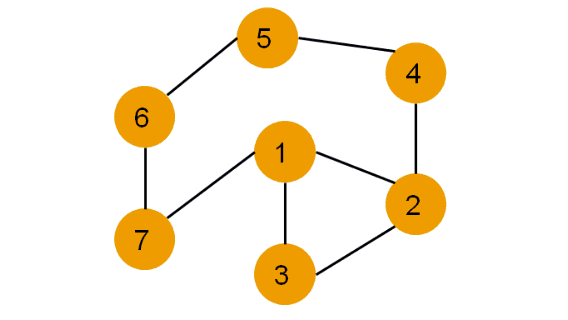
\includegraphics[width=0.5\linewidth]{image.png}
    \caption{Пример графа на 7 вершинах и 8 рёбрах}
    \label{fig:graph} 
\end{figure}

\subsection*{Упражнения}
\begin{enumerate}
    \item Волшебная страна Фарг почти вся состоит из непреодолимых гор и рек. В ней есть шесть городов: А, Б, В, Г, Д и Е. Известно, что из А проложены дороги в Б и Г, из Б — в А, Г и Д, из В — в Г и Е, из Г — в В и Д, из Д — в Б и Г, из Е — только в В. Все остальные дороги непроходимы.
    \begin{enumerate}
        \item Нарисуйте карту страны Фарг.
        \item Нарисуйте карту так, чтобы дороги не пересекались.
        \item Может ли житель города А попасть в город Д, если ему нельзя проходить через Г?
        \item Сможет ли он при тех же условиях попасть в город Е?
    \end{enumerate}
    \item Между девятью планетами Солнечной системы введено космическое сообщение. Ракеты летают по следующим маршрутам: Земля – Меркурий, Плутон – Венера, Земля – Плутон, Плутон – Меркурий, Меркурий – Венера, Уран – Нептун, Нептун – Сатурн, Сатурн – Юпитер, Юпитер – Марс и Марс – Уран. Можно ли добраться с Земли до Марса?
    \item В стране Цифра есть 9 городов с названиями 1, 2, 3, 4, 5, 6, 7, 8, 9. Путешественник обнаружил, что два города соединены авиалинией в том и только в том случае, если двузначное число, составленное из цифр-названий этих городов, делится на 3. Можно ли добраться из города 1 в город 9?
\end{enumerate}

\subsection*{Полезные факты}
\begin{enumerate}
    \item \textbf{(Лемма о рукопожатиях)} Сумма степеней вершин чётна и равно удвоенному числу рёбер.
    \item \textbf{(Следствие)} В любом графе число вершин нечетной степени четно.
    \item \textbf{(Число рёбер в полном графе)} Если в полном графе $n$ вершин, то в нём $ \frac{n(n-1)}{2}$ ребёр.
\end{enumerate}
\subsection*{Задачи}
\begin{enumerate}
    \item В деревне 15 телефонов. Можно ли их соединить проводами так, чтобы каждый телефон был соединен ровно с пятью другими? 
    \item В государстве 100 городов, и из каждого из них выходит 4 дороги. Сколько всего дорог в государстве?
    \item В классе 27 человек. Каждая девочка дружит с 5 мальчиками, а каждый мальчик с 4 девочками. Сколько мальчиков в классе?
    \item В Тридевятом царстве лишь один вид транспорта – ковер-самолет. Из столицы выходит 21 ковролиния, из города Дальний – одна, а из всех остальных городов – по 20. Докажите, что из столицы можно долететь в Дальний (возможно, с пересадками).
    \item Каждое из рёбер полного графа с 6 вершинами покрашено в один из двух цветов.
Докажите, что есть три вершины, все рёбра между которыми – одного цвета.
\end{enumerate}

\end{document}
